\documentclass[12pt,letterpaper]{article}
\usepackage{amsmath}
\usepackage{amsfonts}
\usepackage[figurewithin=section,tablewithin=section]{caption}
\usepackage[usenames,dvipsnames]{color}
\usepackage{graphicx}
\usepackage{longtable}
\usepackage{rotating}
\usepackage{booktabs}
\usepackage[bibencoding=utf8, citestyle=authoryear,bibstyle=authoryear,maxbibnames=99]{biblatex}
%\addbibresource{~/Projects/MyBibtex.bib}

\bibliography{/home/jsibert/Projects/MyBibtex.bib,/home/jsibert/MendeleyBibTex/library.bib}


\usepackage[pdftex,bookmarks=false]{hyperref}
\hypersetup{pdfauthor={John Sibert}
            pdfsubject={variable transmission and mortality rate estimates}
            pdftitle={Simple SIR Statistical Model}
            pdfkeywords={COVID-19, SIR Model, random effects, TMB}
            }%

\newcommand\doublespacing{\baselineskip=1.6\normalbaselineskip}
\newcommand\singlespacing{\baselineskip=1.0\normalbaselineskip}
\newcommand\help[1]{\color{Magenta}{\it #1 }\normalcolor}
\newcommand\EG{e.g.\ }
\newcommand\perda{$\rm{da}^{-1}$}

\title{Estimating short term trends in transmission and mortality rates
during the Covid 19 Epidemic}

\author{
John Sibert\thanks{sibert@hawaii.edu; johnrsibert@gmail.com}\\
Joint Institute of Marine and Atmospheric Research\\
University of Hawai`i at M\={a}noa\\
Honolulu, HI  96822 U.S.A.\\[0.125in]
\date{\today}
}

\begin{document}

\maketitle

\doublespacing

\section*{Introduction}

The sudden advent of the COVID-19 pandemic provoked many political
jurisdictions to advise people to ``shelter in place'' and to practice
``social distancing''. If this advice has been effective, it should be
possible to detect the effects of the advice by comparing changes in
numbers of infected people and perhaps changes in transmission rates
over time and
between areas. The SIR models of epidemic spread divide the affected
population into three compartments: 
Susceptible, Infected and Recovered.
SIR models are
usually expressed as coupled ordinary differential equations,
\begin{eqnarray}
\label{eqn:SIR}
\frac{dS}{dt} &=& -\beta\frac{IS}{N} - \mu S\\
\frac{dI}{dt} &=& \hphantom{-}\beta\frac{IS}{N} - \mu I -\gamma I\\
\frac{dR}{dt} &=&  -\mu R +\gamma I\\
N &=& S + I + R
\end{eqnarray}
where $N$ is the population size, $\beta$ is the instantaneous
transmission rate ($[t^{-1}]$), $\mu$ is the instantaneous mortality rate
($[t^{-1}]$),  and $\gamma$ is the instantaneous recovery rate
($[t^{-1}]$).  

%https://en.wikipedia.org/wiki/Compartmental_models_in_epidemiology

Unfortunately, few data sets include data for each of
these compartments. 
The New York Times' ``historical'' 
data\footnote{\label{ff:nyt}\url{https://github.com/nytimes/covid-19-data/}}
is an easily accessible source of data. These
data comprise daily totals of ``cases'' and ``deaths'' for each county
in the United States. I assume that the data included as ``cases'' are
a reasonable approximations of the Infected compartment ($I$) in a SIR model. 
There are simply no credible data of comparable scope on either the Susceptible or
the Recovered compartments.

\section*{Model Structure}
I make some simplifying assumptions in the face of incomplete data: 
(1) The entire population is susceptible so that $S/N = 1$. 
(2) Over the short term, the size of the
Susceptible compartment does not change, 
$\frac{dS}{dt} = 0 = \frac{dN}{dt}$,
eliminating the Susceptible compartment.
(3) People who recover from a COVID-19 infection return to the Susceptible
compartment, eliminating the Recovered compartment. 
With these assumptions, and with the addition of a ``deaths''
compartment, the simplified SIR model is
\begin{eqnarray}
\label{eqn:sSIR}
\frac{dI}{dt} &=&  \beta I - \mu I -\gamma I\\
\frac{dD}{dt} &=& \mu I
\end{eqnarray}
and has state variables that might be matched to available observations.

The data available during the initial stages of the COVID-19 pandemic
contain measurement errors of various types.
Definitions and methods of detecting and reporting the numbers of
infected persons vary between political jurisdictions (or
``geographies'' in the parlance of the New York Times) and may also
change with time.
Comparable uncertainties also occur in reporting of deaths caused
by COVID-19 infection.
There is additional variability in the biosocial
processes that mediate disease transmission.

State-space models separate variability in the biosocial
processes in the system (transition model)
from errors in observing features of interest
in the system (observation model).
(See \cite{Harvey1990}).

The general form of a state-space process or transition model is
\begin{equation}
\alpha_t=T(\alpha_{t-1}) + \eta_t
\end{equation}
where $\alpha_t$ is the state at time $t$ and 
the function $T$ embodies the dynamics mediating the
development of the state at time $t$ from the state at the previous
time with random process error, $\eta_t$.

The transition model for the simplified SIR model is constructed from finite difference
approximations of equation (\ref{eqn:sSIR}) with associated log-normal
random errors.
\begin{eqnarray}
\label{eqn:sSIRfdI}
I_t &=& I_{t-\Delta t}\big(1+\Delta t(\beta_{t-\Delta t} - \mu_{t-\Delta t}
- \gamma_{t-\Delta t})\big)e^{\eta_t}\\
\label{eqn:sSIRfdD}
D_t &=& \big(D_{t-\Delta t} + \Delta t \mu_{t-\Delta t}I_{t-\Delta
t}\big)e^{\eta_t}
\end{eqnarray}
where $\eta$ is a normal random deviate, $\eta\sim
N(0,\sigma_\eta)$, representing temporal variability in the biosocial
factors that mediate the spread of the pandemic. 
The recovery rate, $\gamma_{t-\Delta t}$, in equation
(\ref{eqn:sSIRfdI}) is computed algebraically as
\begin{equation}
\gamma_{t-\Delta t} = \beta_{t-\Delta t} - \mu_{t-\Delta t} +
(1-\frac{I_t}{I_{t-\Delta t}})
\end{equation}
I have no particular
justification, beyond the parsimony principle, for the assumption that
the variance, $\sigma_\eta$, of the processes for $I$ and $D$, should be the
same.

One approach to modeling time-dependent rates of transmission and
mortality, $\beta$ and $\mu$, is to treat them as random effects
(\cite{Skaug2006}). Random effects are appropriate if repeating a time
series of observations would not yield the same outcome as the initial
observations. Random effects are also appropriate when observing
the same process in two different areas. I model the  $\beta$ and
$\mu$ time series as log-normal random walks. I assume that
\begin{eqnarray}
\log\beta_t &=& \log\beta_{t-\Delta t}+\varepsilon;\quad \varepsilon\sim 
N(0,\sigma_\beta)\\
\log\mu_t &=& \log\mu_{t-\Delta t}+\varrho;\quad \varrho\sim
N(0,\sigma_\mu)
\end{eqnarray}

The general form of the state-space observation model is
\begin{equation}
x_t = O(\alpha_t) + \varphi_t
\end{equation}
where the function $O$ describes the measurement process with
error $\varepsilon$ in observing the state $\alpha$.

I applied separate observation error models for cases and
deaths. The observation model for cases is a simple log-normal error
\begin{equation}
\label{eqn:logNlike}
\log\varphi_t = \bigg(\log\frac{1}{\sqrt{2\pi\sigma^2_I}} -\Bigl(\frac{\log
I_t-\log\widehat{I}_t}{\sigma_I}\Bigr)^2\bigg)\\
\end{equation}
where $I$ is the observed number of cases and $\widehat{I}$ is the
number of cases predicted by equation~\ref{eqn:sSIRfdI}.


Not all those afflicted by COVID-19 have died; there are far fewer
deaths than infections. In addition,
the observed time series for both $I$ and $D$ begins at the first recorded
case. The first recorded death occurs several days or weeks after the
first recorded case. 
Therefor the deaths time-series inevitably contains a
substantial number of recorded zeros. 
The observation model for deaths accommodates observed zeroes by
assuming to be ``zero-inflated'' log normal likelihood given by
\begin{equation}
\label{eqn:ZIlogNlike}
  \log \varepsilon_t = \left\{
    \begin{array}{r@{\;:\quad}l}
       D_t > 0 &
(1-p_0)\cdot\bigg(\log\frac{1}{\sqrt{2\pi\sigma^2_D}}
          -\Bigl(\frac{\log D_t-\log\widehat{D}_t}{\sigma_D}\Bigr)^2\bigg)\\
       D_t = 0 & p_0 \cdot\log \frac{1}{\sqrt{2\pi\sigma^2_D}}\\
    \end{array}
  \right.
\end{equation}
where $D$ is the observed number of deaths,
$\widehat{D}$ is the number of deaths predicted by
equation~\ref{eqn:sSIRfdD}, 
and $p_0$ is the proportion of observed deaths equal to zero.


Model parameters are estimated by
maximizing the joint likelihood of the process errors, observation
errors, and random effects.
\begin{equation}
\label{eqn:likelihood}
L(\theta,\alpha,x)=
\prod^m_{t=2}\big[\phi\big(\alpha_t-T(\alpha_{t-1}), \Sigma_\eta\big)\big]\cdot
\prod^m_{t=1}\big[\phi\big(x_t-O(\alpha_t),
\Sigma_\varepsilon\big)\big]
\end{equation}
where $m$ is the number of days elapsed since the first recorded case,
$x_t$ is the vector of daily observations of cases and deaths,
$\alpha_t$ is the vector of the daily calculations of the state
variables and random effects,
and $\theta$ 
is a vector of model parameters (Table~\ref{tab:allvars1}).
The R package TMB (\cite{TMB0000} package was used to 
estimate the parameters of the model. 
The R and supporting C++ files are available on 
github.\footnote{simpleSIR4 at \url{https://github.com/johnrsibert/SIR-Models}}

\begin{table}
\caption{List of model variables for the simple SIR model.
There are two state variables computed from the of estimated
parameters and random effects.
There are two random effects and five estimated variance parameters.
}
\label{tab:allvars1}
\begin{center}
\begin{tabular}{ll}
\hline
Variable & Definition\\
\hline
\hline
       & {\it State variables:}\\
$I$      & Number of infected individuals or ``cases''\\
$D$      & Number of deaths\\
       & {\it Random effects:}\\
$\beta_t$ & Transmission rate\\
$\mu_t$   & Mortality rate\\
       & {\it Estimated parameters:}\\
$\sigma_I$ & Infectious compartment estimation standard deviation\\
$\sigma_D$ & Deaths compartment estimation standard deviation\\
$\sigma_\eta$ & Standard deviation of transmission and deaths process errors\\
$\sigma_\beta$ & Standard deviation of transmission rate random walk\\
$\sigma_\mu$ & Standard deviation of mortality rate random walk\\
\hline
\end{tabular}
\end{center}
\end{table}

\clearpage
\section*{Results}

\begin{figure}
\begin{center}
\includegraphics[width=1.00\textwidth]{../Graphics/counties_per_capita.png}
\end{center}
\caption{\label{fig:percap}
Trends in number of cases per 1000 people in the 30 most populous US
counties.
The vertical gray bar mark the date of the California shelter in place order.
}
\end{figure}

%All data are derived from the New York times github 
%site\footnote{See note \ref{ff:nyt}.}.
% {\url{https://github.com/nytimes/covid-19-data/}}. 

The trends in number of cases in the thirty largest counties in the
United States are shown in Figure~(\ref{fig:percap}).
These trajectories fall into two more or less distinct groups: those
that are concave downward, \EG New York City (NYNY), and those that are
concave upward, \EG Miami-Dade FL (MDFL).

Prevalence histories for these five counties are shown in
Figure~\ref{fig:prev} where the 11-day moving average of the daily
increase in cases demonstrates clearly
the efficacy of control measures.

\begin{figure}
{\scriptsize
\begin{center}
\begin{tabular}{ll}
\multicolumn{1}{c}{New York City}&\multicolumn{1}{c}{Cook Co. IL}\\
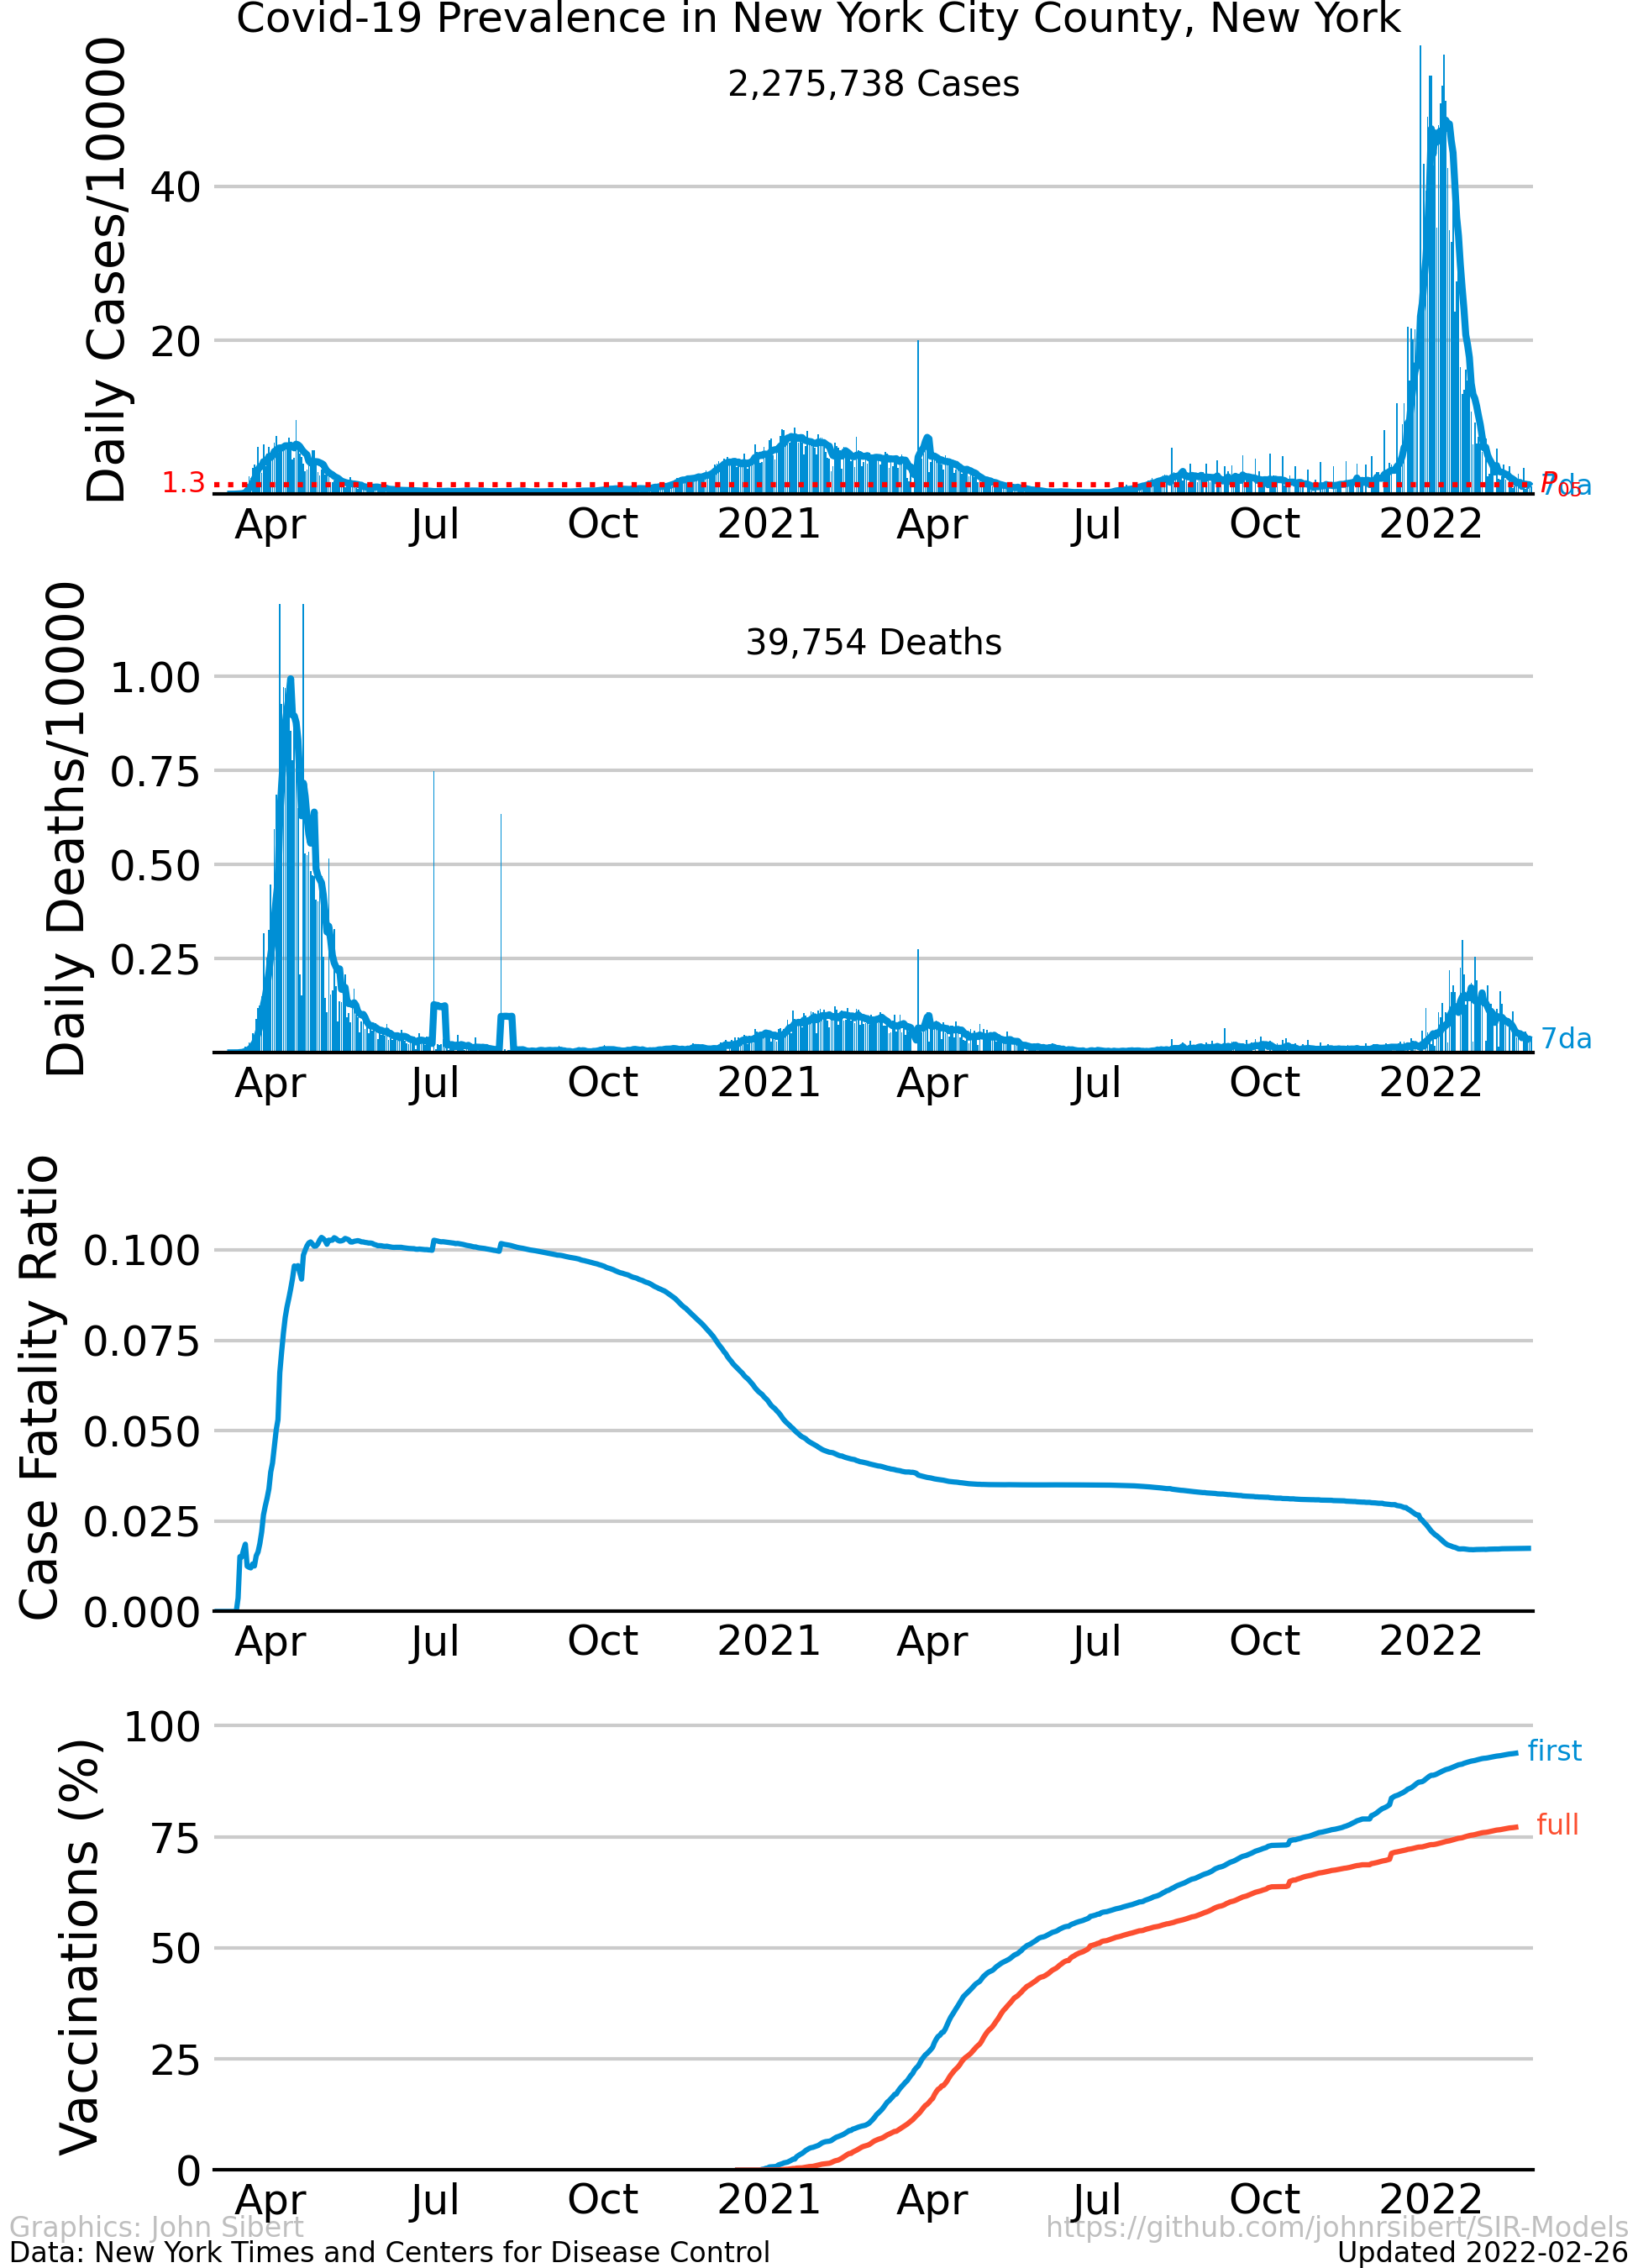
\includegraphics[width=0.50\textwidth]{../Graphics/New_York_CityNY_prevalence.png}&
\includegraphics[width=0.50\textwidth]{../Graphics/CookIL_prevalence.png}\\
\\
\multicolumn{1}{c}{Miami-Dade Co. FL}&\multicolumn{1}{c}{Maricopa Co. AZ}\\
\includegraphics[width=0.50\textwidth]{../Graphics/Miami-DadeFL_prevalence.png}&
\includegraphics[width=0.50\textwidth]{../Graphics/MaricopaAZ_prevalence.png}\\
\\
\multicolumn{1}{c}{Broward Co. FL}&\multicolumn{1}{c}{Honolulu Co. HI}\\
\includegraphics[width=0.50\textwidth]{../Graphics/BrowardFL_prevalence.png}&
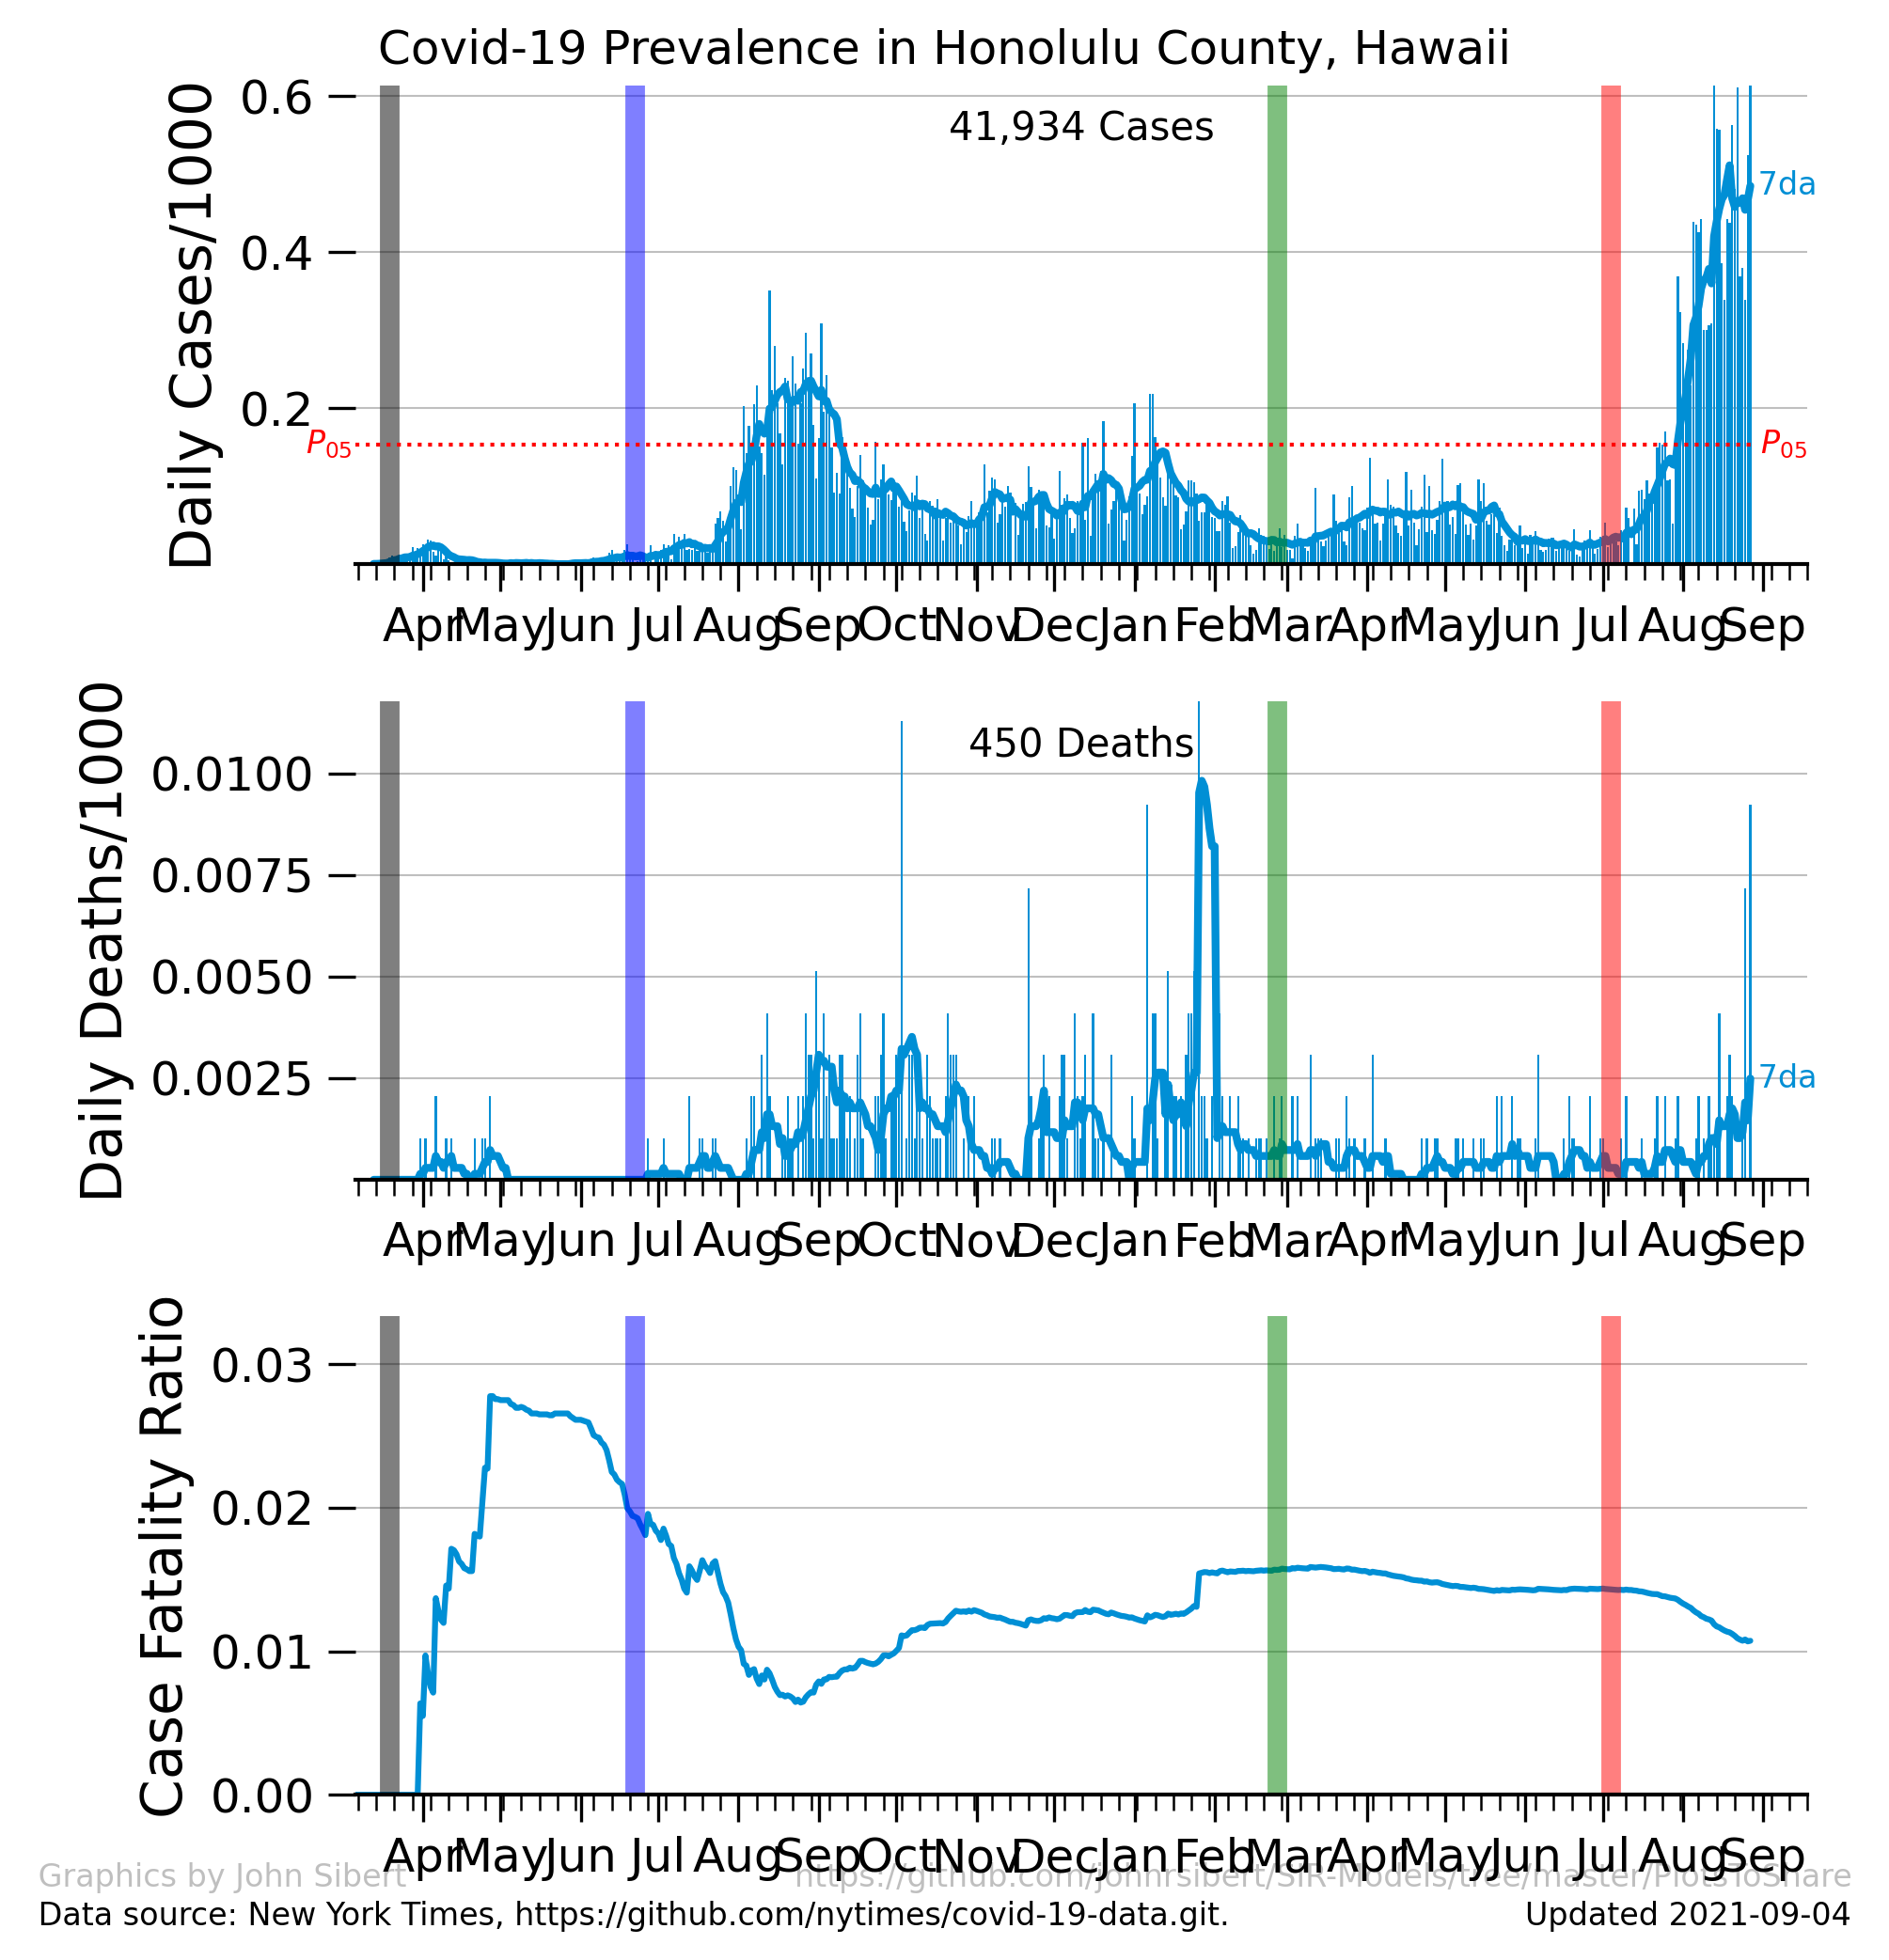
\includegraphics[width=0.50\textwidth]{../Graphics/HonoluluHI_prevalence.png}\\
\end{tabular}
\end{center}
}
\caption{\label{fig:prev}
Prevalence trajectories for six US counties.
Blue bars indicate daily increases increases in cases and deaths;
blue lines indicate 11 day moving averages of daily increases; 
pale blue lines indicate cumulative numbers (labeled $\Sigma C$ and
$\Sigma D$); 
vertical gray bar marks the California shelter in place order.
\help{remove annotations.}
}
\end{figure}

Model results are shown in figures \ref{fig:ests1} and \ref{fig:ests2}.
The model reproduces the observed numbers of cases and deaths almost
exactly.
The `+' symbols in the Cases and Deaths graphs represent the observed
cases ($I$) and deaths ($D$) from the data. 
The red lines overlaying the symbols are model predictions ($\widehat{I}$)
and ($\widehat{D}$) of in cases and deaths. 
$\sigma_I$ and $\sigma_D$ are the estimated standard deviations for
cases and deaths likelihood contributions, equations (\ref{eqn:logNlike}) 
and (\ref{eqn:ZIlogNlike}).
The shaded areas bounded by red outlines are 
$\pm 2$ estimated standard deviations around the estimated trends.
These standard deviations are, in some cases, equivalent to an error of approximately
one case or death.

The solid blue lines in the $\beta$ and $\mu$ plots are the estimated
transmission and death rate random effects.
The shaded areas bounded by blue outlines are
estimated random effects $\pm 2$ standard deviations of the generating
random walks.
The red lines labeled $\tilde{\beta}$ and $\tilde{\mu}$ are the
medians of the two random effects.

The estimated transmission rates are very high
at the beginning of each time series, exceeding 1\perda in Miami-Dade
County, equivalent to a doubling time of less than one day.


\begin{figure}
{\scriptsize
\begin{center}
\begin{tabular}{ll}
\multicolumn{1}{c}{New York City}&\multicolumn{1}{c}{Cook Co. IL}\\
\includegraphics[width=0.50\textwidth]{../Graphics/New_York_CityNY_TMB_estimates.png}&
\includegraphics[width=0.50\textwidth]{../Graphics/CookIL_TMB_estimates.png}\\
\\
\multicolumn{1}{c}{Nassau Co. NY}&\multicolumn{1}{c}{Philadelphia Co.  PA}\\
\includegraphics[width=0.50\textwidth]{../Graphics/NassauNY_TMB_estimates.png}\\
%\includegraphics[width=0.50\textwidth]{../Graphics/PhiladelphiaPA_estimates.png}\\
\end{tabular}
\end{center}
}
\caption{\label{fig:ests1}
}
\end{figure}

\begin{figure}
{\scriptsize
\begin{center}
\begin{tabular}{ll}
\multicolumn{1}{c}{Miami-Dade Co. FL}&\multicolumn{1}{c}{Maricopa Co. AZ}\\
\includegraphics[width=0.50\textwidth]{../Graphics/Miami-DadeFL_TMB_estimates.png}&
\includegraphics[width=0.50\textwidth]{../Graphics/MaricopaAZ_TMB_estimates.png}\\
\\
\multicolumn{1}{c}{Palm Beach Co. FL}&\multicolumn{1}{c}{Travis Co. TX}\\
\includegraphics[width=0.50\textwidth]{../Graphics/Palm_BeachFL_TMB_estimates.png}\\
%\includegraphics[width=0.50\textwidth]{../Graphics/TravisTX_estimates.png}\\
\end{tabular}
\end{center}
}
\caption{\label{fig:ests2}
}
\end{figure}


\begin{sidewaystable}
\caption{\label{tab:sumres}
Model results.
Estimating $\beta$ and $\mu$ trends as random effects with computed $\gamma$.
Data updateed from https://github.com/nytimes/covid-19-data.git
2020-07-17.
}
\centering
{\small
%%%%%%%%%%%%%%

\begin{tabular}{lrrrrrrrrrrrr}
\hline
 County            &   $n$ &   $p_0$ &   $f$ &   $C$ &   $\sigma_\eta$ &   $\sigma_\beta$ &   $\sigma_\mu$ &   $\sigma_I$ &   $\sigma_D$ &   $\tilde\gamma$ &   $\tilde{\beta}$ &   $\tilde{\mu}$ \\
\hline
 Nassau, NY        & 133   &  0.0896 & -3590 &     1 &          0.183  &          0.142   &       0.00157  &       0.188  &     0.0105   &       -2.18e-08  &           0.00290 &        0.000322 \\
 New York City, NY & 137   &  0.0942 & -2180 &    10 &          0.298  &          0.0421  &       0.00251  &       0.118  &     0.0739   &       -3.39e-08  &           0.00726 &        0.00043  \\
 Honolulu, HI      & 132   &  0.188  & -3680 &    10 &          0.272  &          0.0236  &       0.00108  &       0.265  &     0.246    &       -6.07e-08  &           0.0179  &        8.69e-05 \\
 Cook, IL          & 174   &  0.303  & -2770 &    10 &          0.38   &          0.022   &       0.000955 &       0.246  &     0.251    &       -2.29e-07  &           0.0278  &        0.000436 \\
 Harris, TX        & 133   &  0.104  & -1900 &    10 &          0.241  &          0.0299  &       0.000958 &       0.282  &     0.253    &       -3.76e-08  &           0.0304  &        0.000292 \\
 Palm Beach, FL    & 126   &  0.0787 & -3940 &     1 &          0.155  &          0.0529  &       0.00502  &       0.105  &     0.0014   &       -2.42e-08  &           0.0310  &        0.000647 \\
 Miami-Dade, FL    & 127   &  0.125  & -1750 &     1 &          0.157  &          0.0551  &       0.000877 &       0.071  &     0.000445 &       -2e-08     &           0.0320  &        0.000638 \\
 Tarrant, TX       & 128   &  0.0775 & -1850 &    10 &          0.273  &          0.0298  &       0.00105  &       0.263  &     0.21     &       -4.01e-08  &           0.0369  &        0.000409 \\
 Broward, FL       & 132   &  0.0827 & -1610 &    10 &          0.208  &          0.0199  &       0.00194  &       0.254  &     0.24     &       -3.17e-08  &           0.0371  &        0.000473 \\
 Travis, TX        & 125   &  0.111  & -2390 &    10 &          0.397  &          0.0236  &       0.0024   &       0.241  &     0.0643   &       -2.91e-08  &           0.0375  &        0.000363 \\
 Dallas, TX        & 128   &  0.0698 & -1520 &    10 &          0.222  &          0.0222  &       0.00186  &       0.277  &     0.177    &       -2.73e-08  &           0.0382  &        0.000622 \\
 Hillsborough, FL  & 137   &  0.181  & -1940 &    10 &          0.113  &          0.219   &       0.00477  &       0.0562 &     0.0309   &       -8.13e-08  &           0.0401  &        0.000599 \\
 Maricopa, AZ      & 172   &  0.312  & -2040 &    10 &          0.213  &          0.0206  &       0.00164  &       0.258  &     0.213    &       -4.26e-07  &           0.0423  &        0.00164  \\
 Bexar, TX         & 155   &  0.25   & -2370 &    10 &          0.199  &          0.0391  &       0.00103  &       0.237  &     0.246    &       -8.51e-08  &           0.0448  &        0.000363 \\
\hline
 Median            & 132.5 &  0.1075 & -2110 &    10 &          0.2175 &          0.02985 &       0.001605 &       0.2435 &     0.1935   &       -3.575e-08 &           0.03445 &        0.000433 \\
\hline
\end{tabular}

%%%%%%%%%%%%%%%%
}\end{sidewaystable}

\clearpage
\section*{Discussion}

Whether the available data are sufficiently informative to enable
estimation of the model parameters is a critical aspect of the
evaluation of any statistical model.
The speed at which the COVID-19 pandemic spread during the first
quarter of
2020 means that the length of the time series doubled during
the development of this model. The capability of the
model improve conveniently during the model development period,
but whether the improvement is
attributable to changes in model structure or to the increase in the
length of the time series is unclear. This ambiguity influenced the
development of the model.

\cite{Sibert2017,Nielsen2014b,Chen2020}

\clearpage
\printbibliography[title=References]

\end{document}
\clearpage

\begin{figure}
\begin{center}
\includegraphics[width=1.00\textwidth]{../Graphics/New_York_CityNY_TMB_estimates.png}
\end{center}
\caption{\label{fig:NYCest}
Model results for New York City.
}
\end{figure}

\begin{figure}
{\scriptsize
\begin{center}
\begin{tabular}{ll}
\multicolumn{1}{c}{Miami-Dade Co. FL}&\multicolumn{1}{c}{ Honolulu Co.  HI}\\
\includegraphics[width=0.50\textwidth]{../Graphics/Miami-DadeFL_TMB_estimates.png}&
\includegraphics[width=0.50\textwidth]{../Graphics/HonoluluHI_TMB_estimates.png}\\
\multicolumn{1}{c}{Alameda Co. CA}&\multicolumn{1}{c}{Dallas Co. TX}\\
\includegraphics[width=0.50\textwidth]{../Graphics/AlamedaCA_TMB_estimates.png}&
\includegraphics[width=0.50\textwidth]{../Graphics/DallasTX_TMB_estimates.png}\\
\end{tabular}
\end{center}
}
\caption{\label{fig:notests}
}
\end{figure}
%%%%%%%%%%%%%%%%%%%%%%%%%%%%%%%%%%%%%%%%%%%%


\begin{figure}
\begin{center}
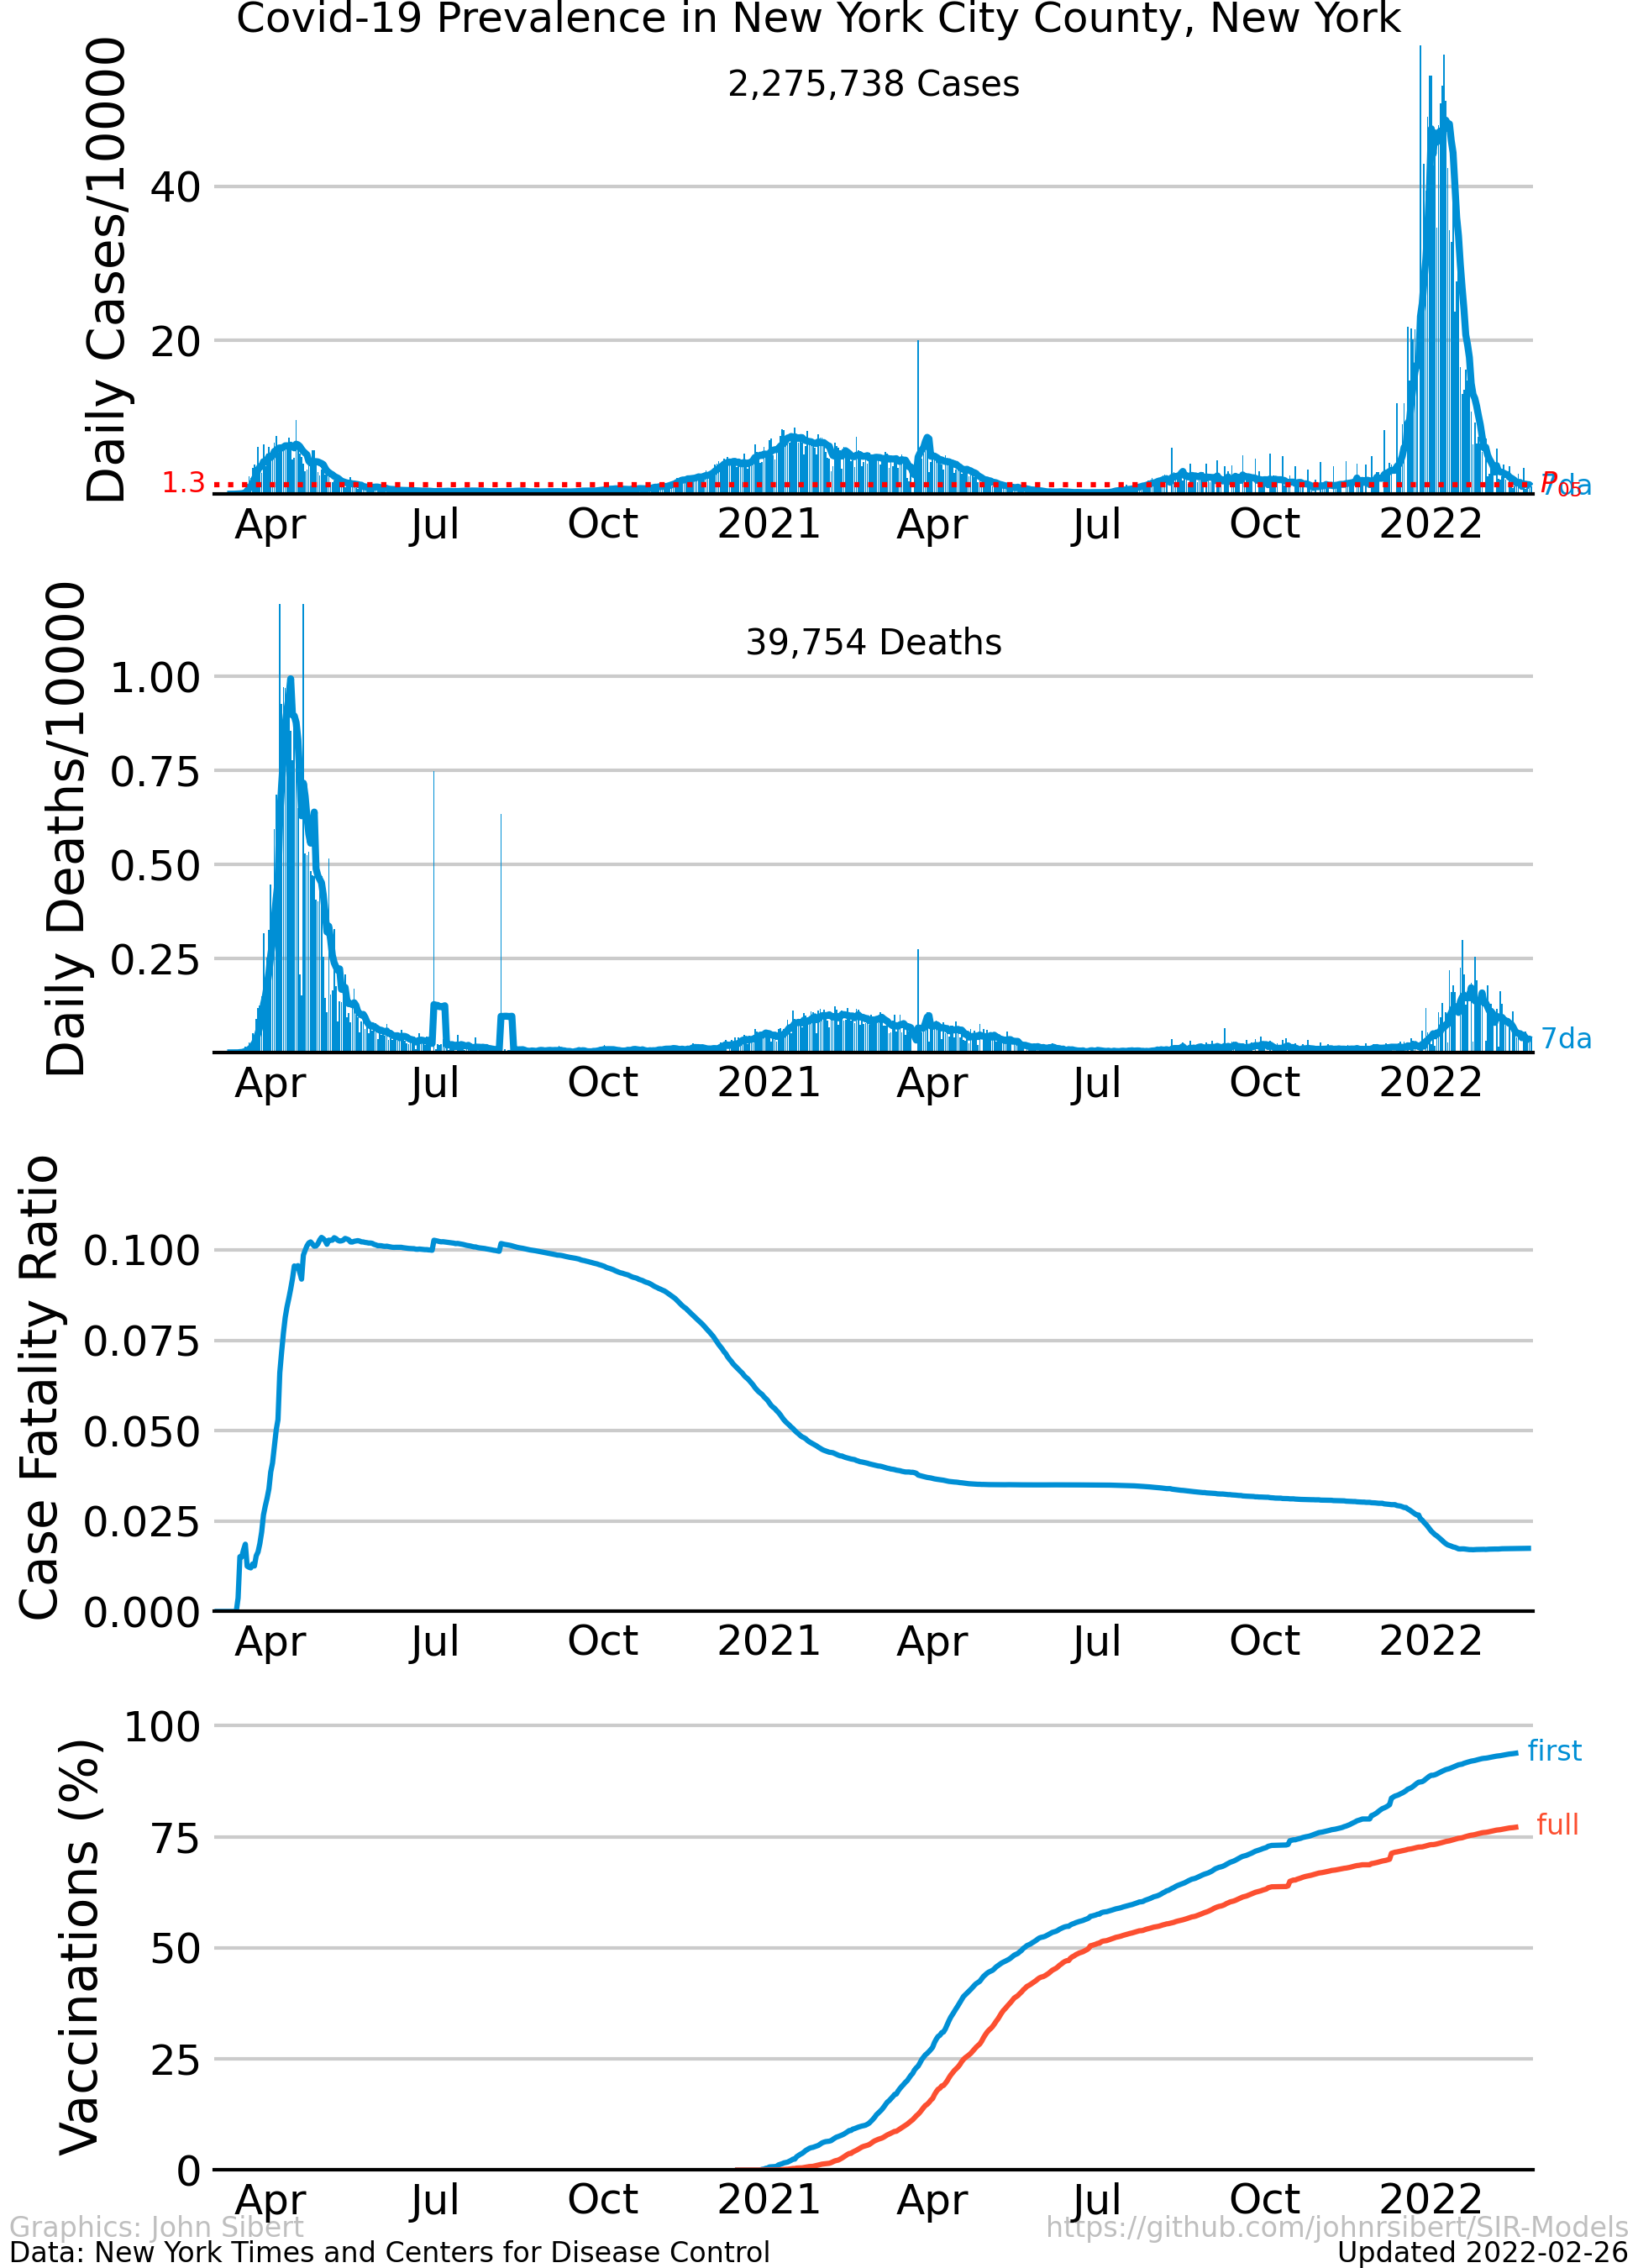
\includegraphics[width=1.00\textwidth]{../Graphics/New_York_CityNY_prevalence.png}
\end{center}
\caption{\label{fig:NYC}
Example effective suppression of transmission, New York City.
Thick blue line indicates cumulative numbers; blue bars indicate daily
increases; thin blue and orange lines indicate 5 and 14 day moving
averages of daily increases; vertical gray bar marks the California
shelter in place decree.
\help{Change ordinates}
}
\end{figure}


\begin{figure}
\begin{center}
\includegraphics[width=1.00\textwidth]{../Graphics/Miami-DadeFL_prevalence.png}
\end{center}
\caption{\label{fig:MDFL}
Effective suppression of transmission and followed by
uncontrolled increase in number of new cases 
Captions as in figure \ref{fig:NYC}.
}
\end{figure}

\begin{figure}
\begin{center}
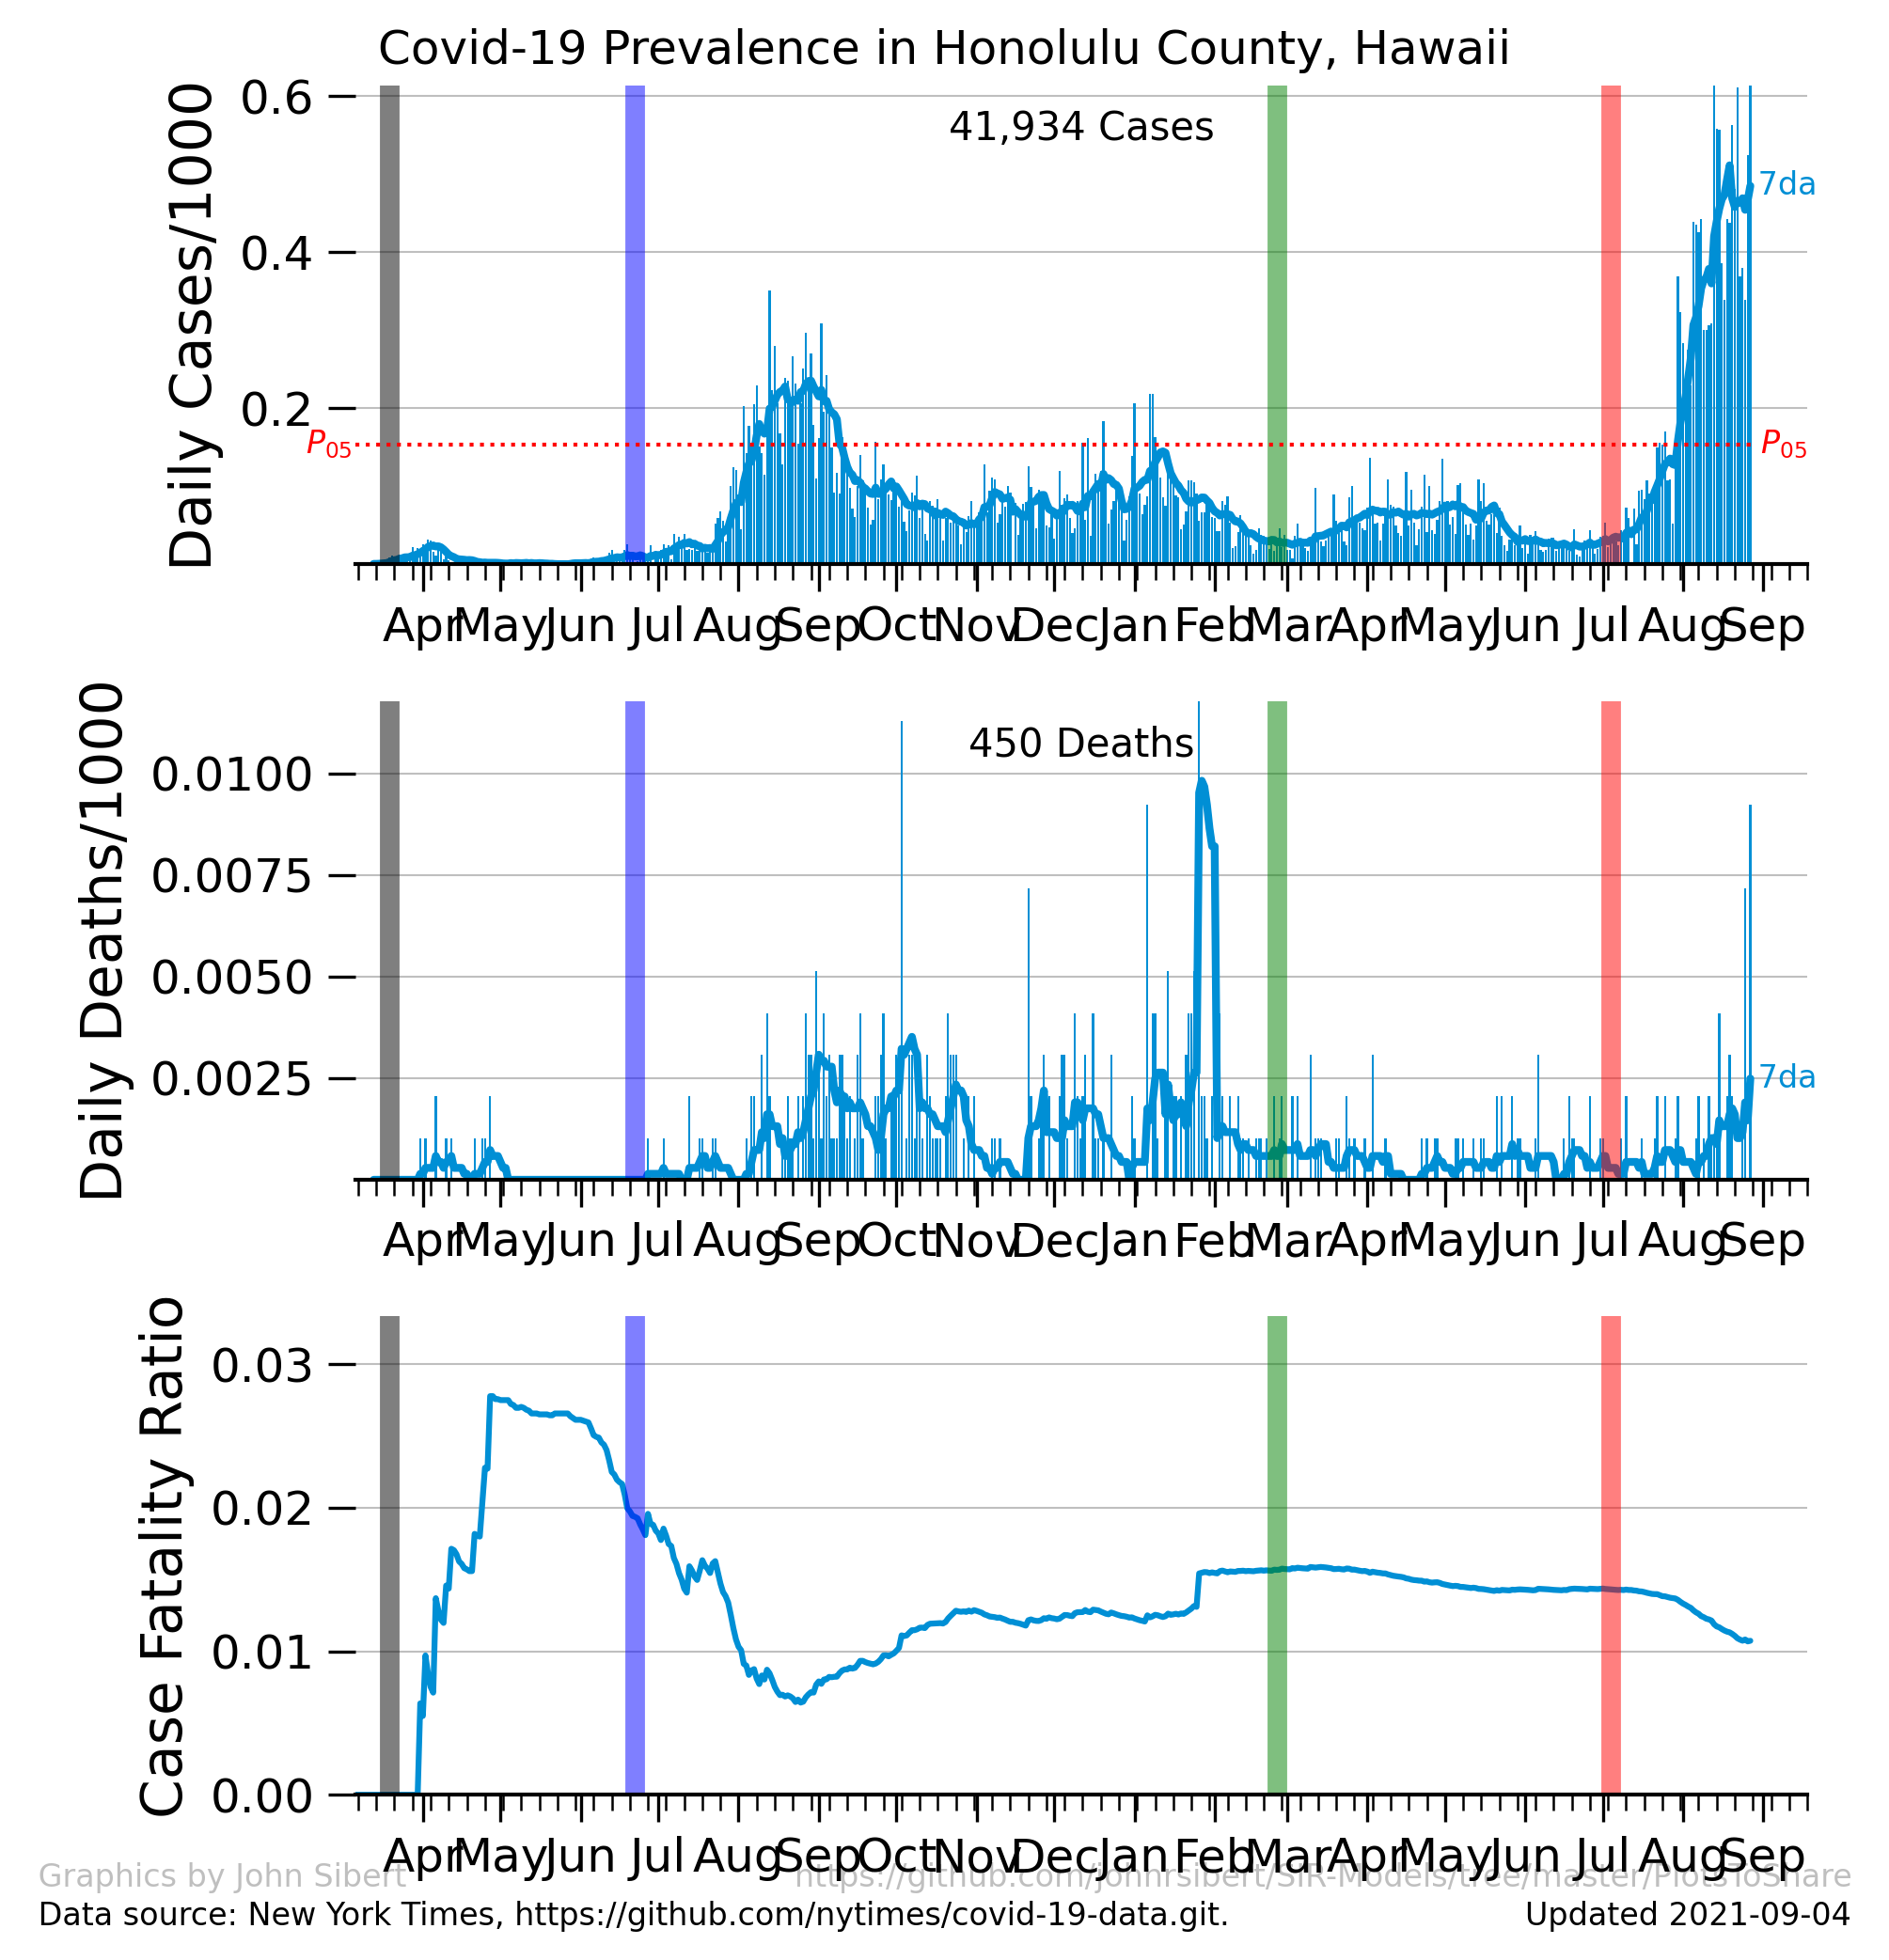
\includegraphics[width=1.00\textwidth]{../Graphics/HonoluluHI_prevalence.png}
\end{center}
\caption{\label{fig:HNL}
Effective suppression of transmission and followed by
uncontrolled increase in number of new cases 
Captions as in figure \ref{fig:NYC}.
}
\end{figure}

\begin{figure}
\begin{center}
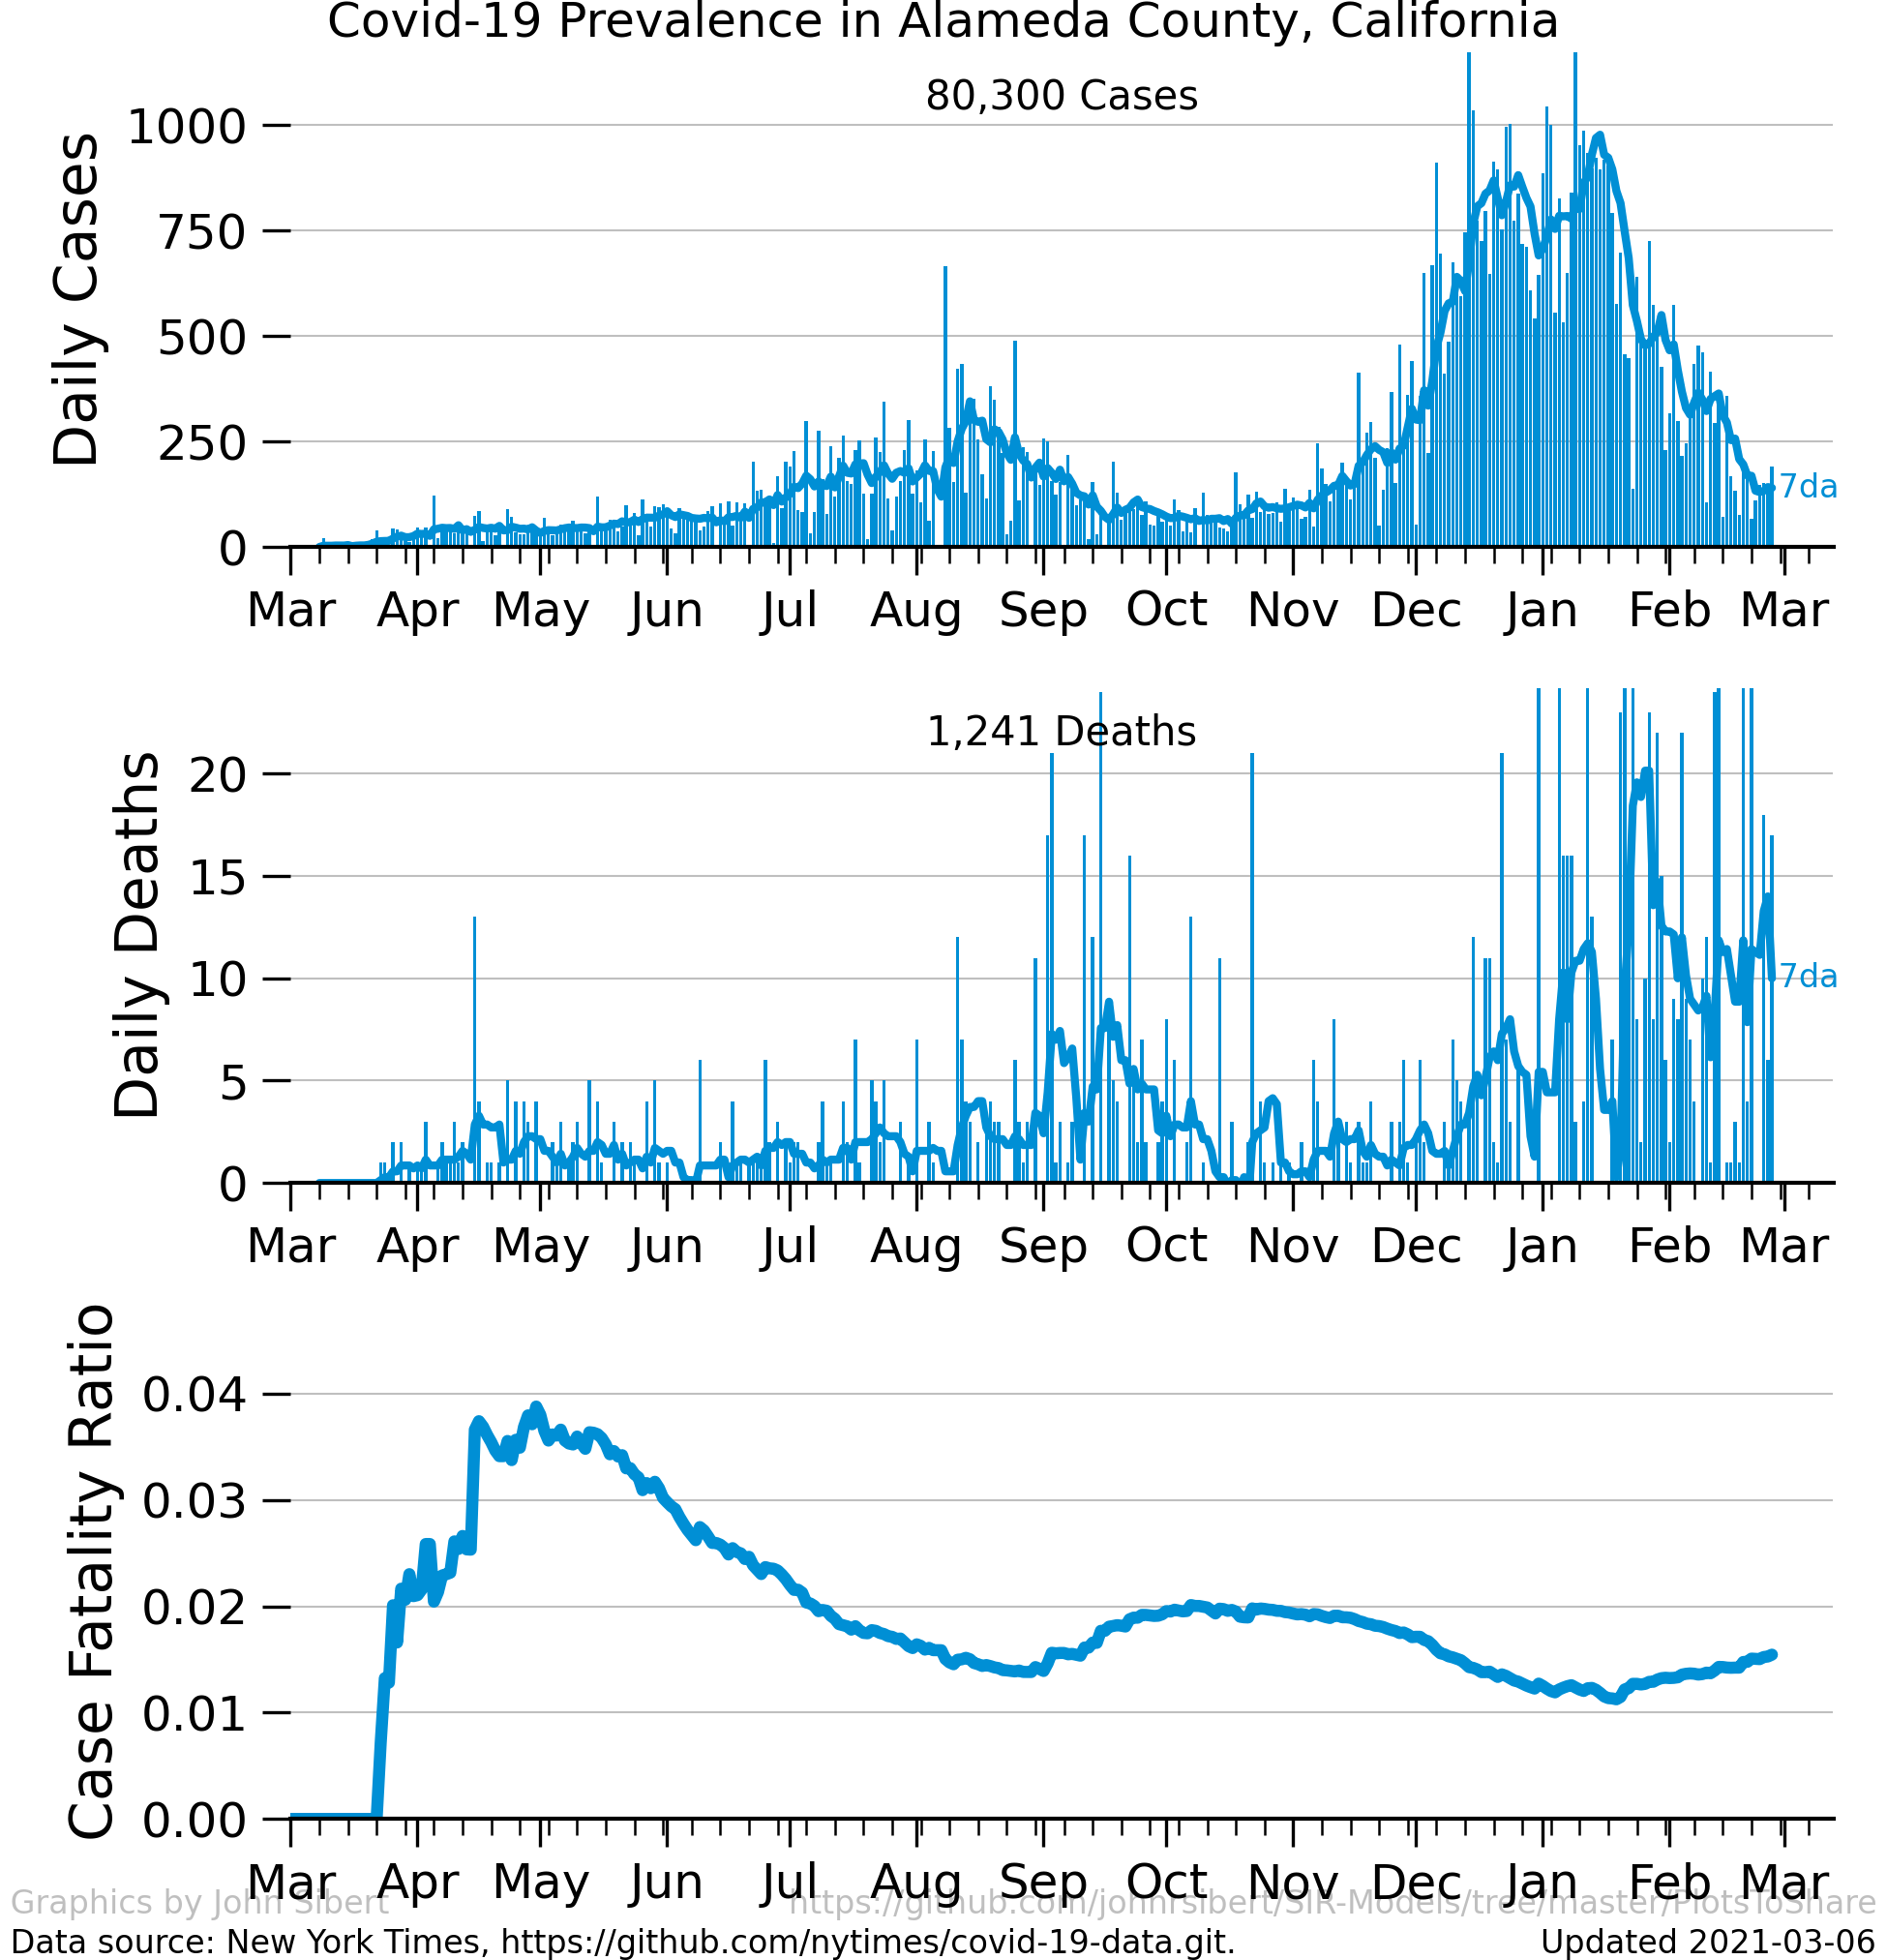
\includegraphics[width=1.00\textwidth]{../Graphics/AlamedaCA_prevalence.png}
\end{center}
\caption{\label{fig:ACA}
Slow monotonic increase in number of new cases.
Captions as in figure \ref{fig:NYC}.
}
\end{figure}

\begin{figure}
\begin{center}
\includegraphics[width=1.00\textwidth]{../Graphics/DallasTX_prevalence.png}
\end{center}
\caption{\label{fig:DTX}
Partial suppression of transmission followed by 
uncontrolled increase in number of new cases.
Captions as in figure \ref{fig:NYC}.
}
\end{figure}

